% CVPR-style milestone report for ARIN 5203.
\documentclass[10pt,twocolumn,letterpaper]{article}

\usepackage[pagenumbers]{cvpr}
\usepackage{graphicx}
\usepackage{amsmath}
\usepackage{amssymb}
\usepackage{booktabs}
\usepackage[hidelinks]{hyperref}

\def\cvprPaperID{ARIN5203}
\def\confName{ARIN 5203}
\def\confYear{2026}

\begin{document}

\title{Fine-Grained Bird Recognition:\\The Role of Foreground and Background}

\author{Zheng Shisheng\\
{\tt\small 21332987}
\and
Lu Yang\\
{\tt\small 21329126}
}

\maketitle

\begin{abstract}
We study fine-grained recognition of 200 bird species using the
Caltech-UCSD Birds-200-2011 (CUB) dataset. The central question is how the
input region and geometric preprocessing affect recognition: does preserving
the complete annotated bird region improve accuracy, and can any gain be
separated from changes in scale, cropping, and background? We fine-tune an
ImageNet-pretrained ResNet-18 under a fixed train/validation split and compare
three matched conditions: the full image, a 10\%-expanded bird crop followed
by center cropping, and a 10\%-expanded bird crop resized with aspect ratio
preserved and padded to a square. Across three training seeds, the letterbox
condition reaches $74.31\% \pm 0.75\%$ validation Top-1 accuracy, compared
with $70.31\% \pm 1.13\%$ for the full image and $67.44\% \pm 0.05\%$ for
center crop. The official CUB test partition remains untouched. These results
are preliminary. A local control that holds the letterbox geometry fixed
obtains $74.00\% \pm 0.36\%$ with bird regions and $65.25\% \pm 0.44\%$ with
whole images, so foreground localization or target scale is important in this
pipeline, although the background effect is not isolated. The remaining work
will inspect background perturbations and model behavior, then perform one
final held-out test evaluation.
\end{abstract}

\section{Introduction}

Fine-grained visual classification requires distinguishing categories that
share a global shape and differ in localized visual evidence, such as bill
shape, head markings, and wing color. CUB-200-2011 provides an appropriate
controlled setting: it contains 200 bird species, annotated boxes, image labels,
and an official train/test division \cite{wah2011cub}. A high-capacity
pre-trained convolutional network can model small visual differences, but its
predictions may also depend on background scene cues or on image regions that
are discarded by preprocessing.

Our project asks whether focusing computation on the annotated bird region
helps a practical recognition pipeline, and whether the effect survives
changes in input geometry. The working hypothesis is that preserving the
complete bird region will reduce accidental removal of discriminative
parts, but the benefit may depend on bird size and on the amount of retained
context. We therefore treat the center-crop and letterbox conditions as
preprocessing comparisons, not as evidence that background is inherently
harmful.

The milestone contributes a reproducible baseline, a fixed validation protocol,
and a three-seed comparison of three input conditions. It also identifies a
confound in the current best result: the letterbox pipeline removes random
resized cropping during training and center cropping during validation in
addition to changing the bird region. The next phase is designed to separate
these effects and then evaluate the selected model once on the official test
set.

\section{Problem Statement and Data}

\subsection{Dataset and splits}

CUB-200-2011 contains 11,788 images from 200 classes, with 5,994 images in the
official training partition and 5,794 in the official test partition. We keep
the official test partition unopened while developing the method. From the
official training partition, we construct a class-stratified validation split
using seed 42: approximately 20\% of each class is assigned to validation,
producing 4,794 training and 1,200 validation images. All methods use the same
split and the split hash is stored with every result.

Each image has a ground-truth bounding box. In the crop-aware conditions, the
box is expanded by 10\% of its width or height on each side, clipped at the
image boundary, and then passed through the condition-specific geometric
pipeline. This use of an exact box is an additional annotation requirement and
must be stated explicitly when comparing against the unrestricted full-image
setting.

\subsection{Prediction target and metrics}

The model predicts one of 200 species labels. We report Top-1 accuracy, Top-5
accuracy, and Macro-F1 on the fixed validation split. Top-1 measures the main
decision, Top-5 tests whether the correct species remains among the leading
candidates, and Macro-F1 gives each species equal weight rather than allowing
frequent classes to dominate. Means and sample standard deviations summarize
three training seeds (42, 43, and 44); they are not confidence intervals.

\section{Technical Approach}

\subsection{Backbone and training protocol}

We use ResNet-18 with ImageNet-pretrained weights \cite{he2016resnet} and replace
its final fully connected layer with a 200-way classifier. Training uses ten
epochs, batch size 32, AdamW, weight decay $10^{-4}$, and mixed precision. For
the first two epochs, the backbone is frozen and only the classifier is
trained; all parameters are then fine-tuned with learning rates $10^{-3}$ for
the classifier and $10^{-4}$ for the backbone. At each epoch we retain the
checkpoint with the best validation Top-1 accuracy. The same backbone, loss,
optimizer, epoch budget, and split are used across input conditions.

\subsection{Input conditions}

The three preliminary conditions are:

\begin{enumerate}
\item \textbf{Full image.} Training applies random resized cropping and
horizontal flipping; validation applies resize-to-256 followed by a
224$\times$224 center crop.
\item \textbf{Bird center crop.} The 10\%-expanded bird box is extracted and
then undergoes the same legacy training and validation geometry.
\item \textbf{Bird letterbox.} The 10\%-expanded box is resized so that its
longest side is 224 pixels, preserving aspect ratio, and is centered on a
224$\times$224 canvas. The fill color is RGB $(124,116,104)$, close to the
ImageNet normalization mean. Training keeps only a horizontal flip; validation
is deterministic.
\end{enumerate}

The first two conditions provide the previously established baseline and a
crop control. The letterbox condition aims to preserve the complete bird while
avoiding the head or tail truncation that can occur with center cropping.
However, it also changes the training distribution because random resized
cropping is removed. We therefore describe the current comparison as a
pipeline-level result rather than a causal padding ablation.

\subsection{Planned analyses}

We have completed a whole-image letterbox control with the same reduced
augmentation, separating geometric preservation from the use of a bird box.
Next, we will apply controlled background perturbations (blur, occlusion, and
background-only diagnostic inputs) and report accuracy changes by bird-size
stratum. We will inspect Grad-CAM responses and confusion pairs
\cite{selvaraju2017gradcam}, including cases where letterbox improves or
worsens the prediction. Finally, after freezing the configuration, we will
evaluate the selected checkpoint once on the official test partition.

\section{Intermediate Results}

\begin{table}[t]
\centering
\small
\setlength{\tabcolsep}{3pt}
\begin{tabular}{lccc}
\toprule
Condition & Top-1 (\%) & Top-5 (\%) & Macro-F1 (\%) \\
\midrule
Full image & 70.31 $\pm$ 1.13 & 91.42 $\pm$ 0.22 & 70.02 $\pm$ 0.92 \\
Center crop & 67.44 $\pm$ 0.05 & 89.64 $\pm$ 0.10 & 67.06 $\pm$ 0.23 \\
Letterbox & \textbf{74.31 $\pm$ 0.75} & \textbf{93.06 $\pm$ 0.42} & \textbf{73.97 $\pm$ 0.88} \\
\bottomrule
\end{tabular}
\caption{Validation results over three training seeds. Values are mean
$\pm$ sample standard deviation; the standard deviations are not confidence
intervals. The official test set was not used.}
\label{tab:results}
\end{table}

\begin{figure*}[t]
\centering
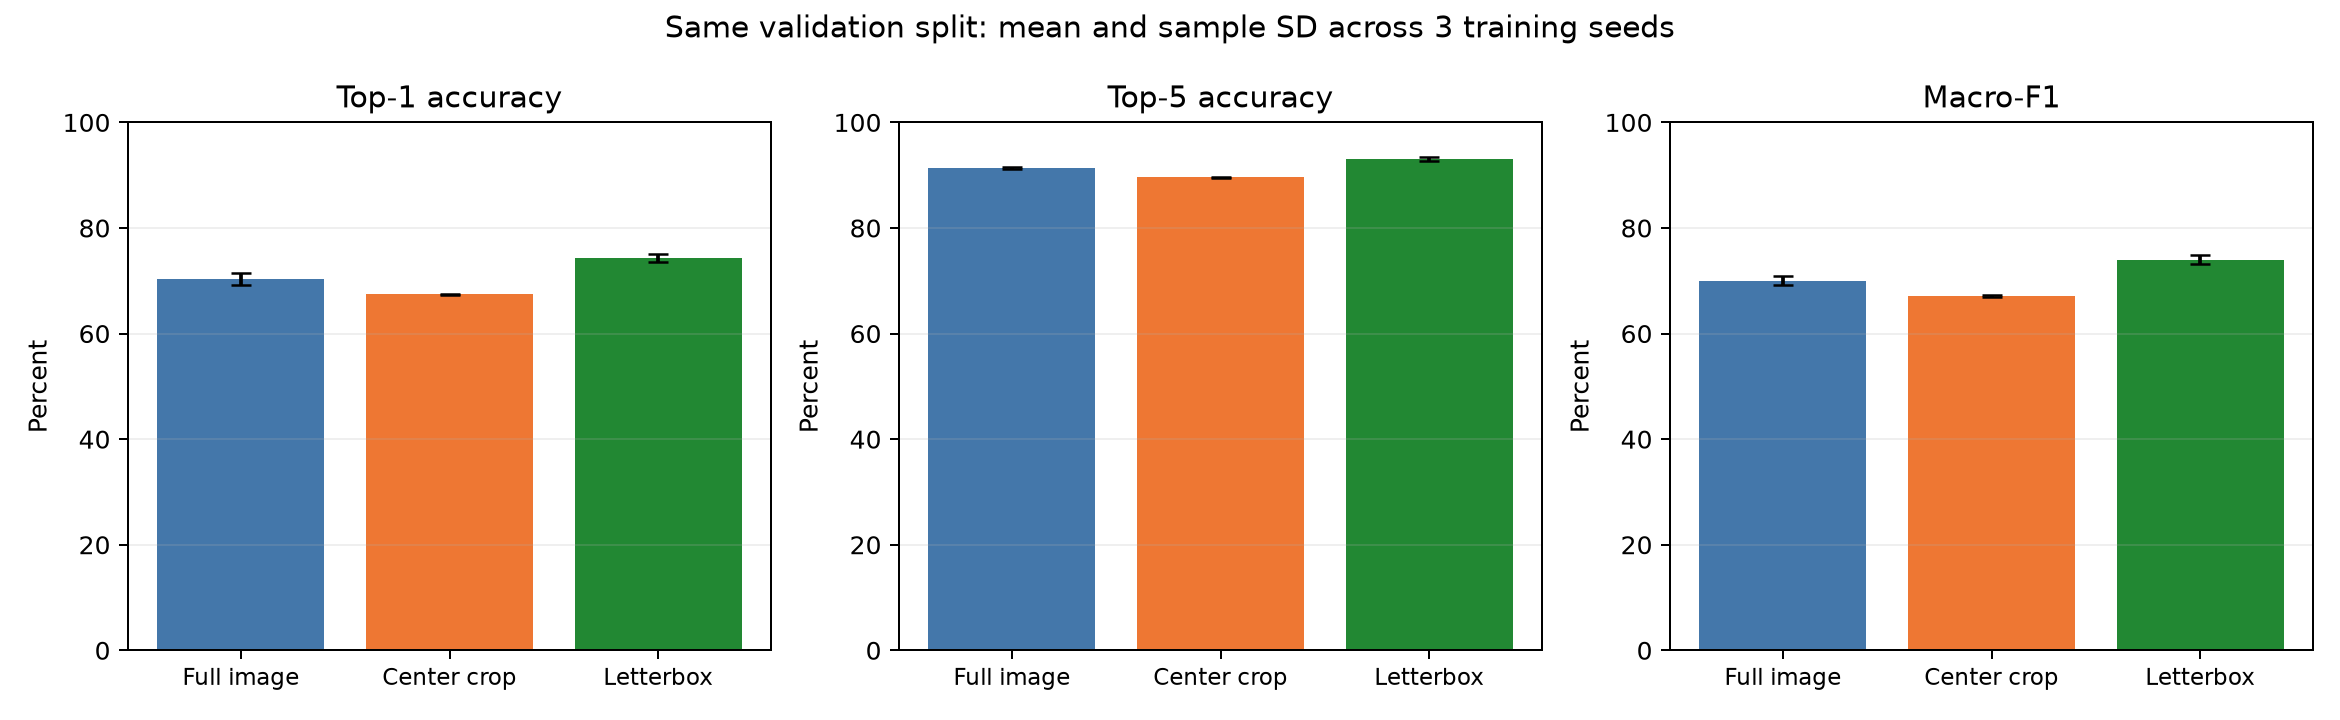
\includegraphics[width=0.92\textwidth]{images/performance_comparison.png}
\caption{Same-validation-set comparison across training seeds 42--44. Error
bars show sample standard deviation, not confidence intervals.}
\label{fig:results}
\end{figure*}

Table~\ref{tab:results} and Figure~\ref{fig:results} summarize the preliminary
comparison. Letterbox obtains the highest mean score on all three metrics and
improves Top-1 by 4.00 percentage points over the full image and by 6.86
points over bird center crop. The direction is consistent across all three
training seeds: paired Top-1 improvements over the full-image condition are
2.75, 4.92, and 4.33 points for seeds 42, 43, and 44, respectively. The lower
within-condition variability of center crop should not be interpreted as
greater generalization, because its mean is substantially lower.

To separate input content from augmentation geometry, whole-image and
bird-region letterbox conditions were each retrained for three seeds on the
same RTX 3060 Laptop GPU with 6~GB memory. The bird-region condition reaches
74.00\% $\pm$ 0.36\% Top-1, while the whole-image condition reaches 65.25\%
$\pm$ 0.44\%. The paired gains are 9.33, 8.08, and 8.83 points for seeds 42,
43, and 44. This rules out removal of random cropping as the sole explanation,
but changing the region also changes target scale and retained background.

The crop-only comparison was negative on average: center crop is 2.86 points
below the full image. This result illustrates why region selection and
geometric processing should be considered together. A narrow crop can remove
context and can also cut off a head, tail, or other fine-grained evidence. In
qualitative inspection, center-cropped inputs sometimes omitted visible parts
of the bird, whereas the letterbox inputs retained the whole expanded region.
These examples are selected for explanation and are not an estimate of the
overall error distribution.

Bird-size stratification suggests that the benefit is not uniform. For images
whose box occupies less than 10\% of the image area ($n=33$), the three-seed
mean Top-1 is 61.62\% for full image, 75.76\% for center crop, and 82.83\% for
letterbox. The sample is small, so this is an exploratory observation rather
than a precise subgroup estimate. For the 10--30\% subgroup ($n=539$),
letterbox averages 73.59\%, compared with 71.06\% for full image and 65.99\%
for center crop.

\section{Discussion and Risks}

The current evidence supports continuing with the region-preserving letterbox
pipeline as the provisional primary method. The whole-image letterbox control
shows that the gain is not explained solely by removing random cropping, but
the crop also increases effective bird scale and removes context. Background
perturbation experiments will provide complementary evidence rather than
definitive causal proof, because artificial occlusion also changes image
statistics.

There are additional limitations. The pipeline assumes that a bird box is
available; an unconstrained upload interface would require automatic
localization or manual annotation. The CUB documentation notes possible image
overlap with ImageNet, so ImageNet pretraining may expose the model to related
images \cite{wah2011cub}. Three seeds provide preliminary stability evidence,
but do not establish statistical significance or deterministic training.
Finally, every reported number is validation performance; opening the test set
before the final configuration is frozen would compromise its role as an
independent evaluation.

\section{Milestone Status and Next Steps}

The data pipeline, model training, checkpointing, validation evaluation, and
three-seed comparison are implemented. The project now has a validated
baseline, a clear preprocessing comparison, and an explicit test-set policy.
The immediate next steps are:

\begin{itemize}
\item separate the background and geometry effects with controlled
perturbations;
\item add Grad-CAM and confusion analysis to explain improvements and failures;
\item freeze the final configuration, evaluate the official test partition
once, and prepare the six-to-eight-page final report.
\end{itemize}

\begin{thebibliography}{9}
\small
\bibitem{wah2011cub}
C. Wah, S. Branson, P. Welinder, P. Perona, and S. Belongie.
\newblock The Caltech-UCSD Birds-200-2011 Dataset.
\newblock \emph{CNS-TR-2011-001}, 2011.

\bibitem{he2016resnet}
K. He, X. Zhang, S. Ren, and J. Sun.
\newblock Deep Residual Learning for Image Recognition.
\newblock In \emph{CVPR}, 2016.

\bibitem{selvaraju2017gradcam}
R. R. Selvaraju, M. Cogswell, A. Das, R. Vedantam, D. Parikh, and D. Batra.
\newblock Grad-CAM: Visual Explanations from Deep Networks via
Gradient-Based Localization.
\newblock In \emph{ICCV}, 2017.

\end{thebibliography}

\end{document}
